\chapter{Release 5:Intégration de l'Intelligence Artificielle}

\DeclareRobustCommand{\greencheck}{%
  \tikz\fill[scale=0.4, color=green]
  (0,.35) -- (.25,0) -- (1,.7) -- (.25,.15) -- cycle;%
}

\minitoc
\section*{Introduction}
\addcontentsline{toc}{section}{Introduction}
Dans le cadre de la septième phase du développement de notre plateforme dédiée aux projets de fin d'études (PFE), nous avons concentré nos efforts sur l'intégration de solutions d'intelligence artificielle avancées. Ces fonctionnalités permettent non seulement de générer des questions d'entretien personnalisées et d'évaluer des réponses en fonction du domaine et du poste recherché, mais aussi de mettre en correspondance intelligemment les offres d'emploi avec les profils des candidats, enrichissant considérablement l'écosystème de notre plateforme.

\section{Objectifs du Sprint 7}

\subsection{Intégration de l'Intelligence Artificielle}
L'objectif principal de ce sprint est de développer et d'intégrer des modules d'intelligence artificielle basés sur des modèles de langage de grande taille (LLM). Ces systèmes doivent permettre :

\begin{itemize}
    \item La génération automatique de questions d'entretien adaptées au domaine et au poste
    \item L'évaluation pertinente des réponses fournies par les candidats
    \item La mise en correspondance intelligente entre CV et offres d'emploi
    \item L'analyse sémantique des compétences et exigences
\end{itemize}

Pour chaque fonctionnalité, nous avons exploré et implémenté deux approches : une première version simple utilisant uniquement le LLM, et une seconde version avancée intégrant une architecture RAG (Retrieval-Augmented Generation) pour des résultats plus personnalisés et contextualisés.

\section{Backlog Fonctionnel – Sprint 7}

\subsection{Backlog Produit – Intelligence Artificielle}
Le tableau ci-dessous recense les user stories associées aux systèmes d'intelligence artificielle. Ces fonctionnalités ont été priorisées selon trois niveaux (Haute, Moyenne, Basse) selon leur impact sur le fonctionnement de l'application.

\begin{table}[H]
\centering
\begin{tabular}{|p{2cm}|p{10cm}|c|}
\hline
\textbf{User Story} & \textbf{Description} & \textbf{Priorité} \\
\hline
US-01 & En tant qu'utilisateur, je veux pouvoir générer des questions d'entretien adaptées à mon domaine professionnel. & Haute \\
\hline
US-02 & En tant qu'utilisateur, je veux pouvoir spécifier le type de poste (stage ou emploi) pour obtenir des questions appropriées. & Haute \\
\hline
US-03 & En tant qu'utilisateur, je veux pouvoir obtenir une évaluation de mes réponses aux questions d'entretien. & Haute \\
\hline
US-04 & En tant qu'utilisateur, je veux recevoir des questions personnalisées en fonction de mon profil et des offres disponibles. & Moyenne \\
\hline
US-05 & En tant qu'administrateur, je veux pouvoir ajouter des documents à la base de connaissances du système. & Moyenne \\
\hline
US-06 & En tant qu'utilisateur, je veux pouvoir visualiser les questions générées de façon claire et organisée. & Haute \\
\hline
US-07 & En tant qu'utilisateur, je veux recevoir des évaluations détaillées sur mes réponses avec des suggestions d'amélioration. & Moyenne \\
\hline
US-08 & En tant qu'étudiant, je veux pouvoir soumettre mon CV pour identifier les offres d'emploi les plus pertinentes. & Haute \\
\hline
US-09 & En tant que recruteur, je veux pouvoir trouver les candidats les plus adaptés à une offre d'emploi spécifique. & Haute \\
\hline
US-10 & En tant qu'utilisateur, je veux obtenir un score de correspondance et des explications détaillées pour les matchs CV-offres. & Moyenne \\
\hline
\end{tabular}
\caption{User Stories liées au système d'intelligence artificielle}
\end{table}

\section{Étude comparative des modèles LLM}
Dans le cadre de notre projet, nous avons mené une analyse approfondie pour sélectionner le modèle LLM le plus adapté à nos besoins. Cette étude comparative a considéré plusieurs critères essentiels tels que la performance, les ressources requises, la confidentialité des données et les restrictions d'utilisation.

\subsection{Critères de sélection}
Pour notre plateforme, nous avons évalué les modèles selon les critères suivants :
\begin{itemize}
    \item \textbf{Performance} : capacité à générer des réponses pertinentes et précises
    \item \textbf{Ressources requises} : exigences matérielles pour l'exécution du modèle
    \item \textbf{Confidentialité} : garanties concernant la protection des données utilisateur
    \item \textbf{Licence} : conditions d'utilisation et restrictions commerciales
    \item \textbf{Facilité d'intégration} : simplicité de déploiement dans notre architecture
\end{itemize}

\subsection{Modèles évalués}
Nous avons analysé trois modèles majeurs du marché :

\subsubsection{GPT-3.5 (OpenAI)}
GPT-3.5 est un modèle très performant développé par OpenAI. Cependant, son utilisation présente plusieurs inconvénients pour notre contexte :
\begin{itemize}
    \item Nécessite une connexion cloud payante avec un système de facturation à l'utilisation
    \item Pose des enjeux de confidentialité car les données transitent par des serveurs externes
    \item Les informations envoyées pourraient potentiellement être enregistrées ou analysées
    \item Incompatible avec nos exigences de protection des données et de souveraineté numérique
\end{itemize}

\subsubsection{LLaMA 2 (Meta)}
LLaMA 2 est un modèle open-source développé par Meta. Son évaluation a révélé :
\begin{itemize}
    \item Performances élevées mais exigences matérielles importantes (GPU très puissants)
    \item Utilisation commerciale restreinte par une licence imposée par Meta
    \item Demande d'accès préalable nécessaire
    \item Conditions spécifiques selon la taille de l'organisation utilisatrice
    \item Déploiement complexifié dans un cadre professionnel, notamment pour les startups
\end{itemize}

\subsubsection{Mistral 7B}
Mistral 7B est un modèle open-source plus récent qui a attiré notre attention par ses caractéristiques avantageuses :
\begin{itemize}
    \item Excellente performance (plus de 64\% sur le benchmark MMLU)
    \item Véritablement open-source sans restriction forte
    \item Code source et poids du modèle librement accessibles et modifiables
    \item Utilisation commerciale autorisée sans demande préalable
    \item Relativement léger (fonctionne avec 16 à 32 Go de VRAM)
    \item Optimisé pour les tâches conversationnelles rapides
\end{itemize}

\subsection{Choix final : Mistral 7B}
Après cette évaluation approfondie, notre choix s'est porté sur Mistral 7B pour les raisons suivantes :
\begin{itemize}
    \item \textbf{Performance} : Score de 64\% sur MMLU, démontrant sa capacité à comprendre et raisonner sur des sujets variés
    \item \textbf{Confidentialité} : Déploiement local possible, garantissant que les données restent sous notre contrôle
    \item \textbf{Économie} : Absence de frais d'utilisation récurrents liés à des API externes
    \item \textbf{Légèreté} : Fonctionnement possible sur des infrastructures modestes
    \item \textbf{Liberté d'utilisation} : Aucune restriction commerciale significative
\end{itemize}

Le benchmark MMLU (Massive Multitask Language Understanding) est particulièrement pertinent car il mesure la capacité du modèle à comprendre et raisonner sur 57 tâches différentes couvrant des domaines variés comme les mathématiques, le droit, la médecine et l'histoire. Le score de 64\% obtenu par Mistral 7B le positionne parmi les meilleurs modèles open-source, prouvant sa polyvalence et sa qualité en tant qu'assistant conversationnel intelligent.

\section{Architecture microservices et intégration}
Le développement de notre solution IA a été abordé selon deux axes principaux : un système de génération et d'évaluation de questions d'entretien, et un système de matching entre CV et offres d'emploi. Pour chacun de ces axes, nous avons d'abord développé une version simple utilisant directement le LLM, puis une version avancée intégrant une architecture RAG (Retrieval-Augmented Generation) pour des résultats plus personnalisés et contextualisés.

En accord avec l'architecture microservices globale de notre plateforme, le module d'intelligence artificielle a été conçu comme un microservice dédié, entièrement intégré à notre backend existant. Toutes les API du système d'IA sont exposées via notre API Gateway principale, assurant ainsi une cohérence d'accès et une sécurité unifiée avec le reste de l'application.

\subsection{Système de questions d'entretien}

\subsubsection{Version sans RAG}
La première version de notre système de génération et d'évaluation de questions d'entretien repose sur une approche directe utilisant uniquement le modèle Mistral 7B. Cette architecture comprend plusieurs composants interconnectés :

\begin{itemize}
    \item \textbf{Ollama} : Plateforme open-source qui simplifie le déploiement local de LLMs comme Mistral. Ollama gère automatiquement le téléchargement, le chargement en mémoire et les interactions avec le modèle.
    
    \item \textbf{Microservice FastAPI Python} : Service API dédié à l'IA qui expose des endpoints pour interagir avec le modèle Mistral. Ce service est intégré à notre architecture microservices globale et accessible via l'API Gateway centrale.
    
    \item \textbf{Backend Node.js} : Service principal de notre application qui communique avec le microservice IA et transmet les données entre l'interface utilisateur et le modèle d'IA.
    
    \item \textbf{Frontend} : Interface utilisateur permettant aux utilisateurs de sélectionner leur domaine et type de poste, et d'afficher les questions générées ou les évaluations reçues.
\end{itemize}

Le microservice IA expose deux endpoints principaux via notre API Gateway :
\begin{itemize}
    \item \texttt{/generate-question/} : Génère des questions d'entretien basées sur le domaine et le niveau spécifiés
    \item \texttt{/evaluate-answer/} : Évalue les réponses fournies par l'utilisateur et peut proposer une question suivante
\end{itemize}
\begin{figure}
    \centering
    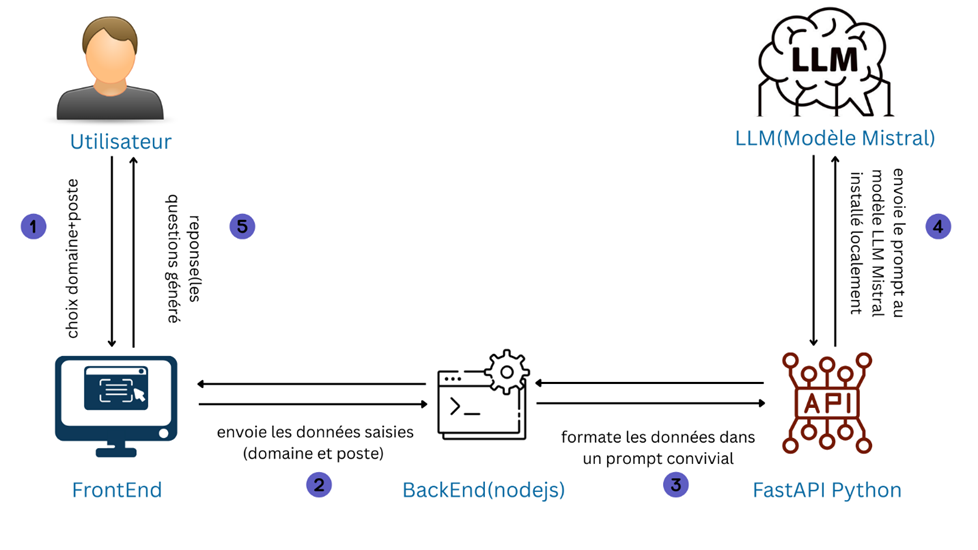
\includegraphics[width=1\linewidth]{images/architecturesansrag.png}
    \caption{Architecture Sans RAG pour les questions / évaluation}
    \label{fig:enter-label}
\end{figure}
\newpage
Le flux de données pour cette version sans RAG suit ce processus :

\begin{enumerate}
    \item L'utilisateur sélectionne son domaine (ex : intelligence artificielle, cloud, flutter) et le niveau (stage ou travail) via l'interface web.
    \item Ces données sont envoyées sous forme de requête HTTP à l'API Gateway.
    \item L'API Gateway route la requête vers le microservice IA.
    \item Le microservice prépare un prompt formaté incluant le domaine et le niveau pour générer une question pertinente.
    \item Le prompt est envoyé au modèle Mistral via Ollama.
    \item Le modèle Mistral génère une question et la renvoie au microservice.
    \item Le microservice formate la réponse en JSON et la renvoie via l'API Gateway.
    \item Les données traversent le backend Node.js qui les relaie à l'interface utilisateur.
    \item La question générée s'affiche à l'écran pour l'utilisateur.
\end{enumerate}

\subsubsection{Version avec RAG pour les questions}
Pour améliorer la pertinence et le contexte des questions générées, nous avons également développé une version RAG de notre système de questions d'entretien. Cette approche enrichit les prompts envoyés au modèle LLM avec des informations précises et ciblées issues de documents internes :
\begin{figure}
    \centering
    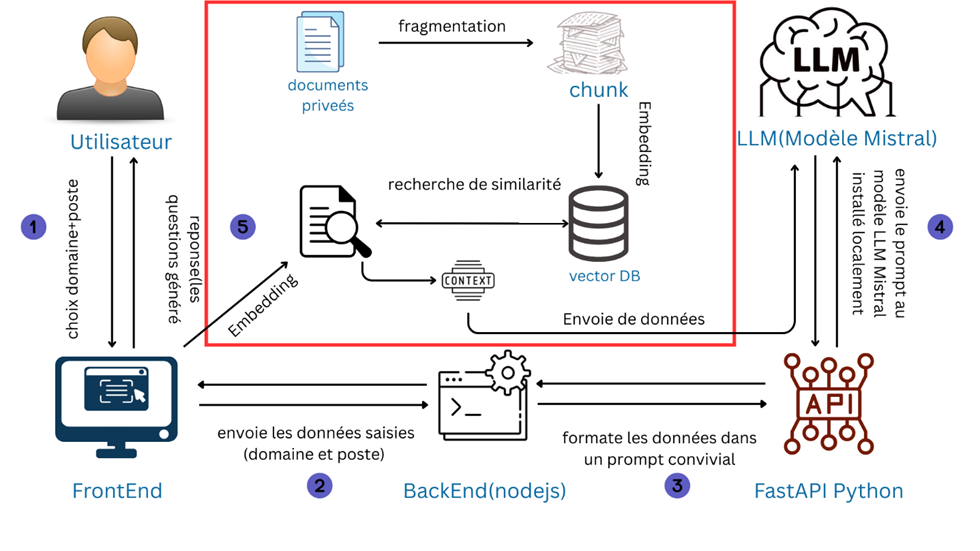
\includegraphics[width=1\linewidth]{images/architectureRAG.png}
    \caption{Architecture IA RAG avec Microservice}
    \label{fig:architecture_RAG}
\end{figure}

\begin{itemize}
    \item \textbf{Corpus de connaissances} : Collection de documents pertinents comme des descriptions de cours, des programmes de formation, des fiches de postes internes et des comptes-rendus d'entretiens précédents.
    
    \item \textbf{Modèle d'embedding} : Convertit les documents et requêtes utilisateurs en vecteurs numériques capturant leur contenu sémantique.
    
    \item \textbf{Base de données vectorielle} : Stocke les vecteurs des documents et permet une recherche par similarité sémantique.
    
    \item \textbf{Sélection de contexte} : Identifie les passages les plus pertinents en fonction du domaine et du niveau demandés par l'utilisateur.
    
    \item \textbf{Prompt enrichi} : Intègre les passages sélectionnés dans le prompt envoyé au modèle Mistral.
\end{itemize}

Cette version avec RAG génère des questions beaucoup plus spécifiques et contextualisées, alignées sur le contenu pédagogique de notre plateforme et les exigences réelles du marché du travail. Le flux de données est similaire à la version sans RAG, mais inclut des étapes supplémentaires de recherche et enrichissement de contexte.


\subsection{Comparaison entre l'approche simple et l'approche RAG pour le matching CV-emploi}

\subsubsection{Diagramme de performance}

\begin{figure}[H]
    \centering
    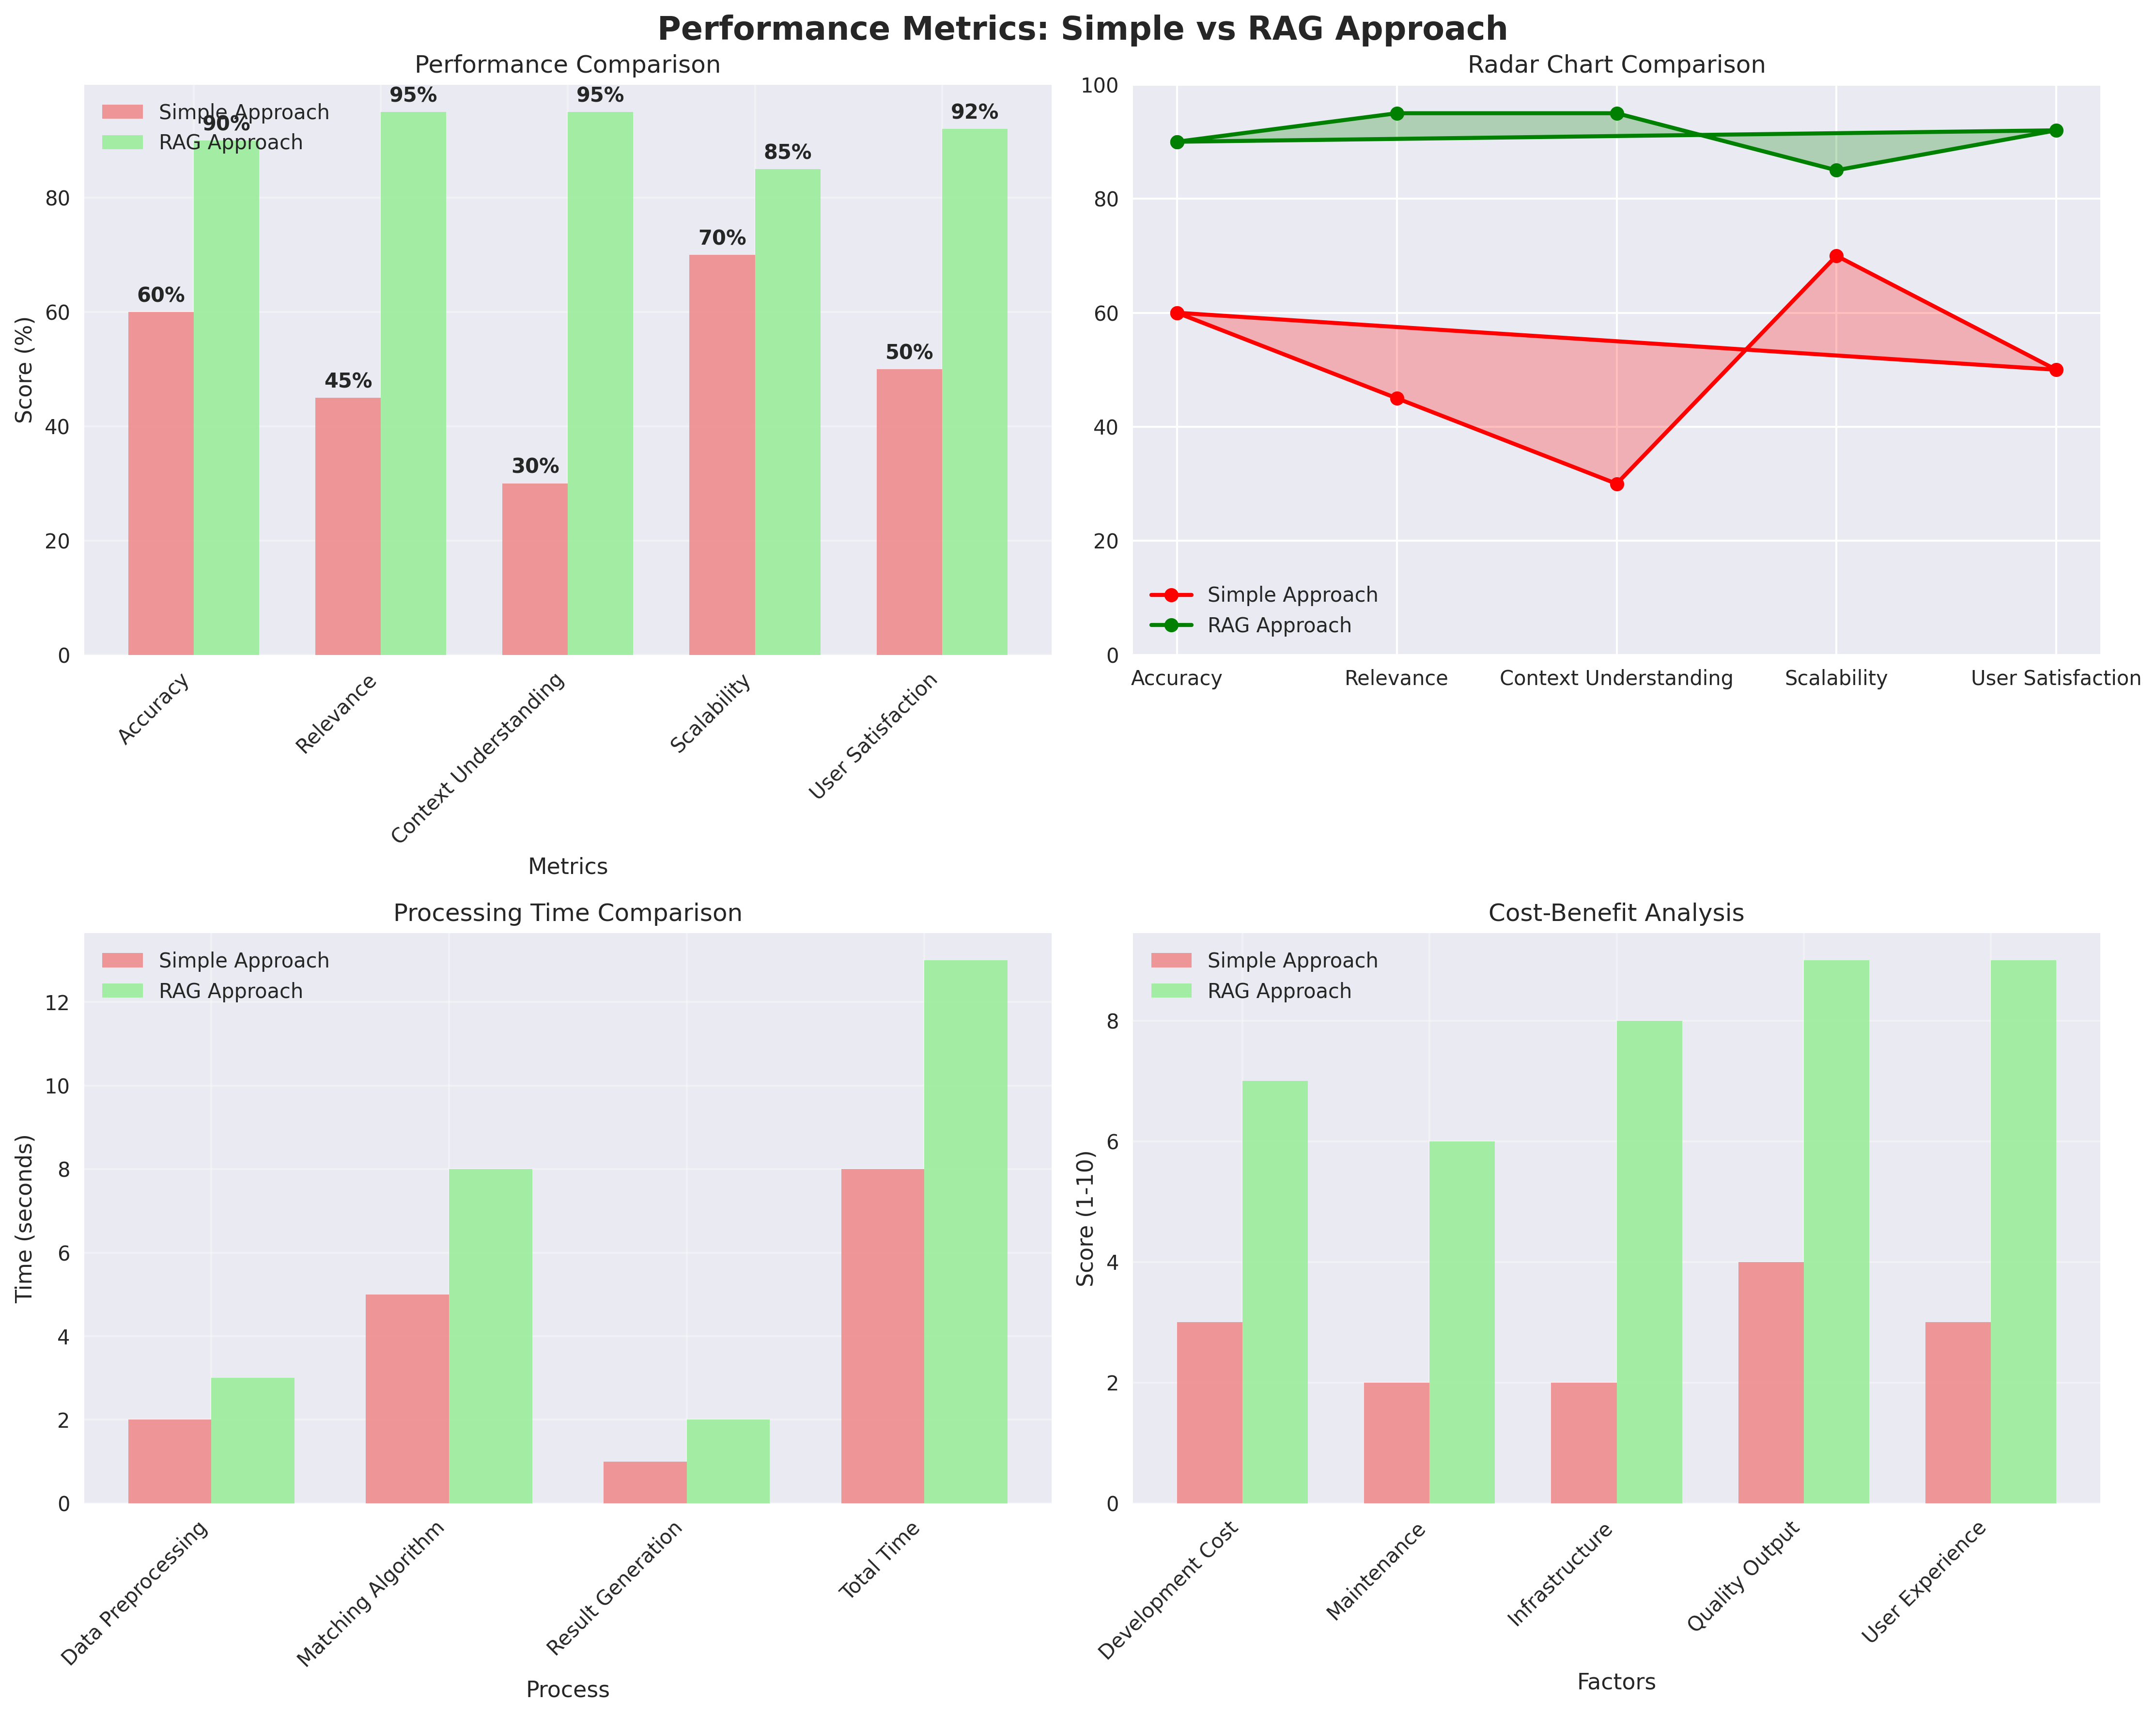
\includegraphics[width=0.9\textwidth]{images/performance_metrics.png}
    \caption{Comparaison des métriques de performance entre approche simple et RAG}
\end{figure}

Ce diagramme compare l'approche simple et l'approche RAG à travers quatre visualisations :

\begin{itemize}
    \item \textbf{Graphique 1 – Métriques principales} : 
    \begin{itemize}
        \item Précision : 60\% (simple) vs 90\% (RAG), soit une amélioration de +50\%.
        \item Pertinence : 45\% vs 95\%, soit +111\%.
        \item Compréhension du contexte : 30\% vs 95\%, soit +217\%.
        \item Scalabilité : 70\% vs 85\%, soit +21\%.
        \item Satisfaction utilisateur : 50\% vs 92\%, soit +84\%.
    \end{itemize}
    
    \item \textbf{Graphique 2 – Radar des performances} : la zone verte (RAG) recouvre entièrement la zone rouge (approche simple), montrant la supériorité de RAG sur tous les critères.
    
    \item \textbf{Graphique 3 – Temps de traitement et qualité} : RAG prend plus de temps (13s vs 8s), mais fournit une qualité 3 fois supérieure, justifiant l'investissement en ressources.
    
    \item \textbf{Graphique 4 – Coûts et ROI} : Malgré des coûts plus élevés, RAG offre un retour sur investissement favorable grâce à sa qualité de matching accrue.
\end{itemize}

\subsubsection{Diagramme des bonnes pratiques}

\begin{figure}[H]
    \centering
    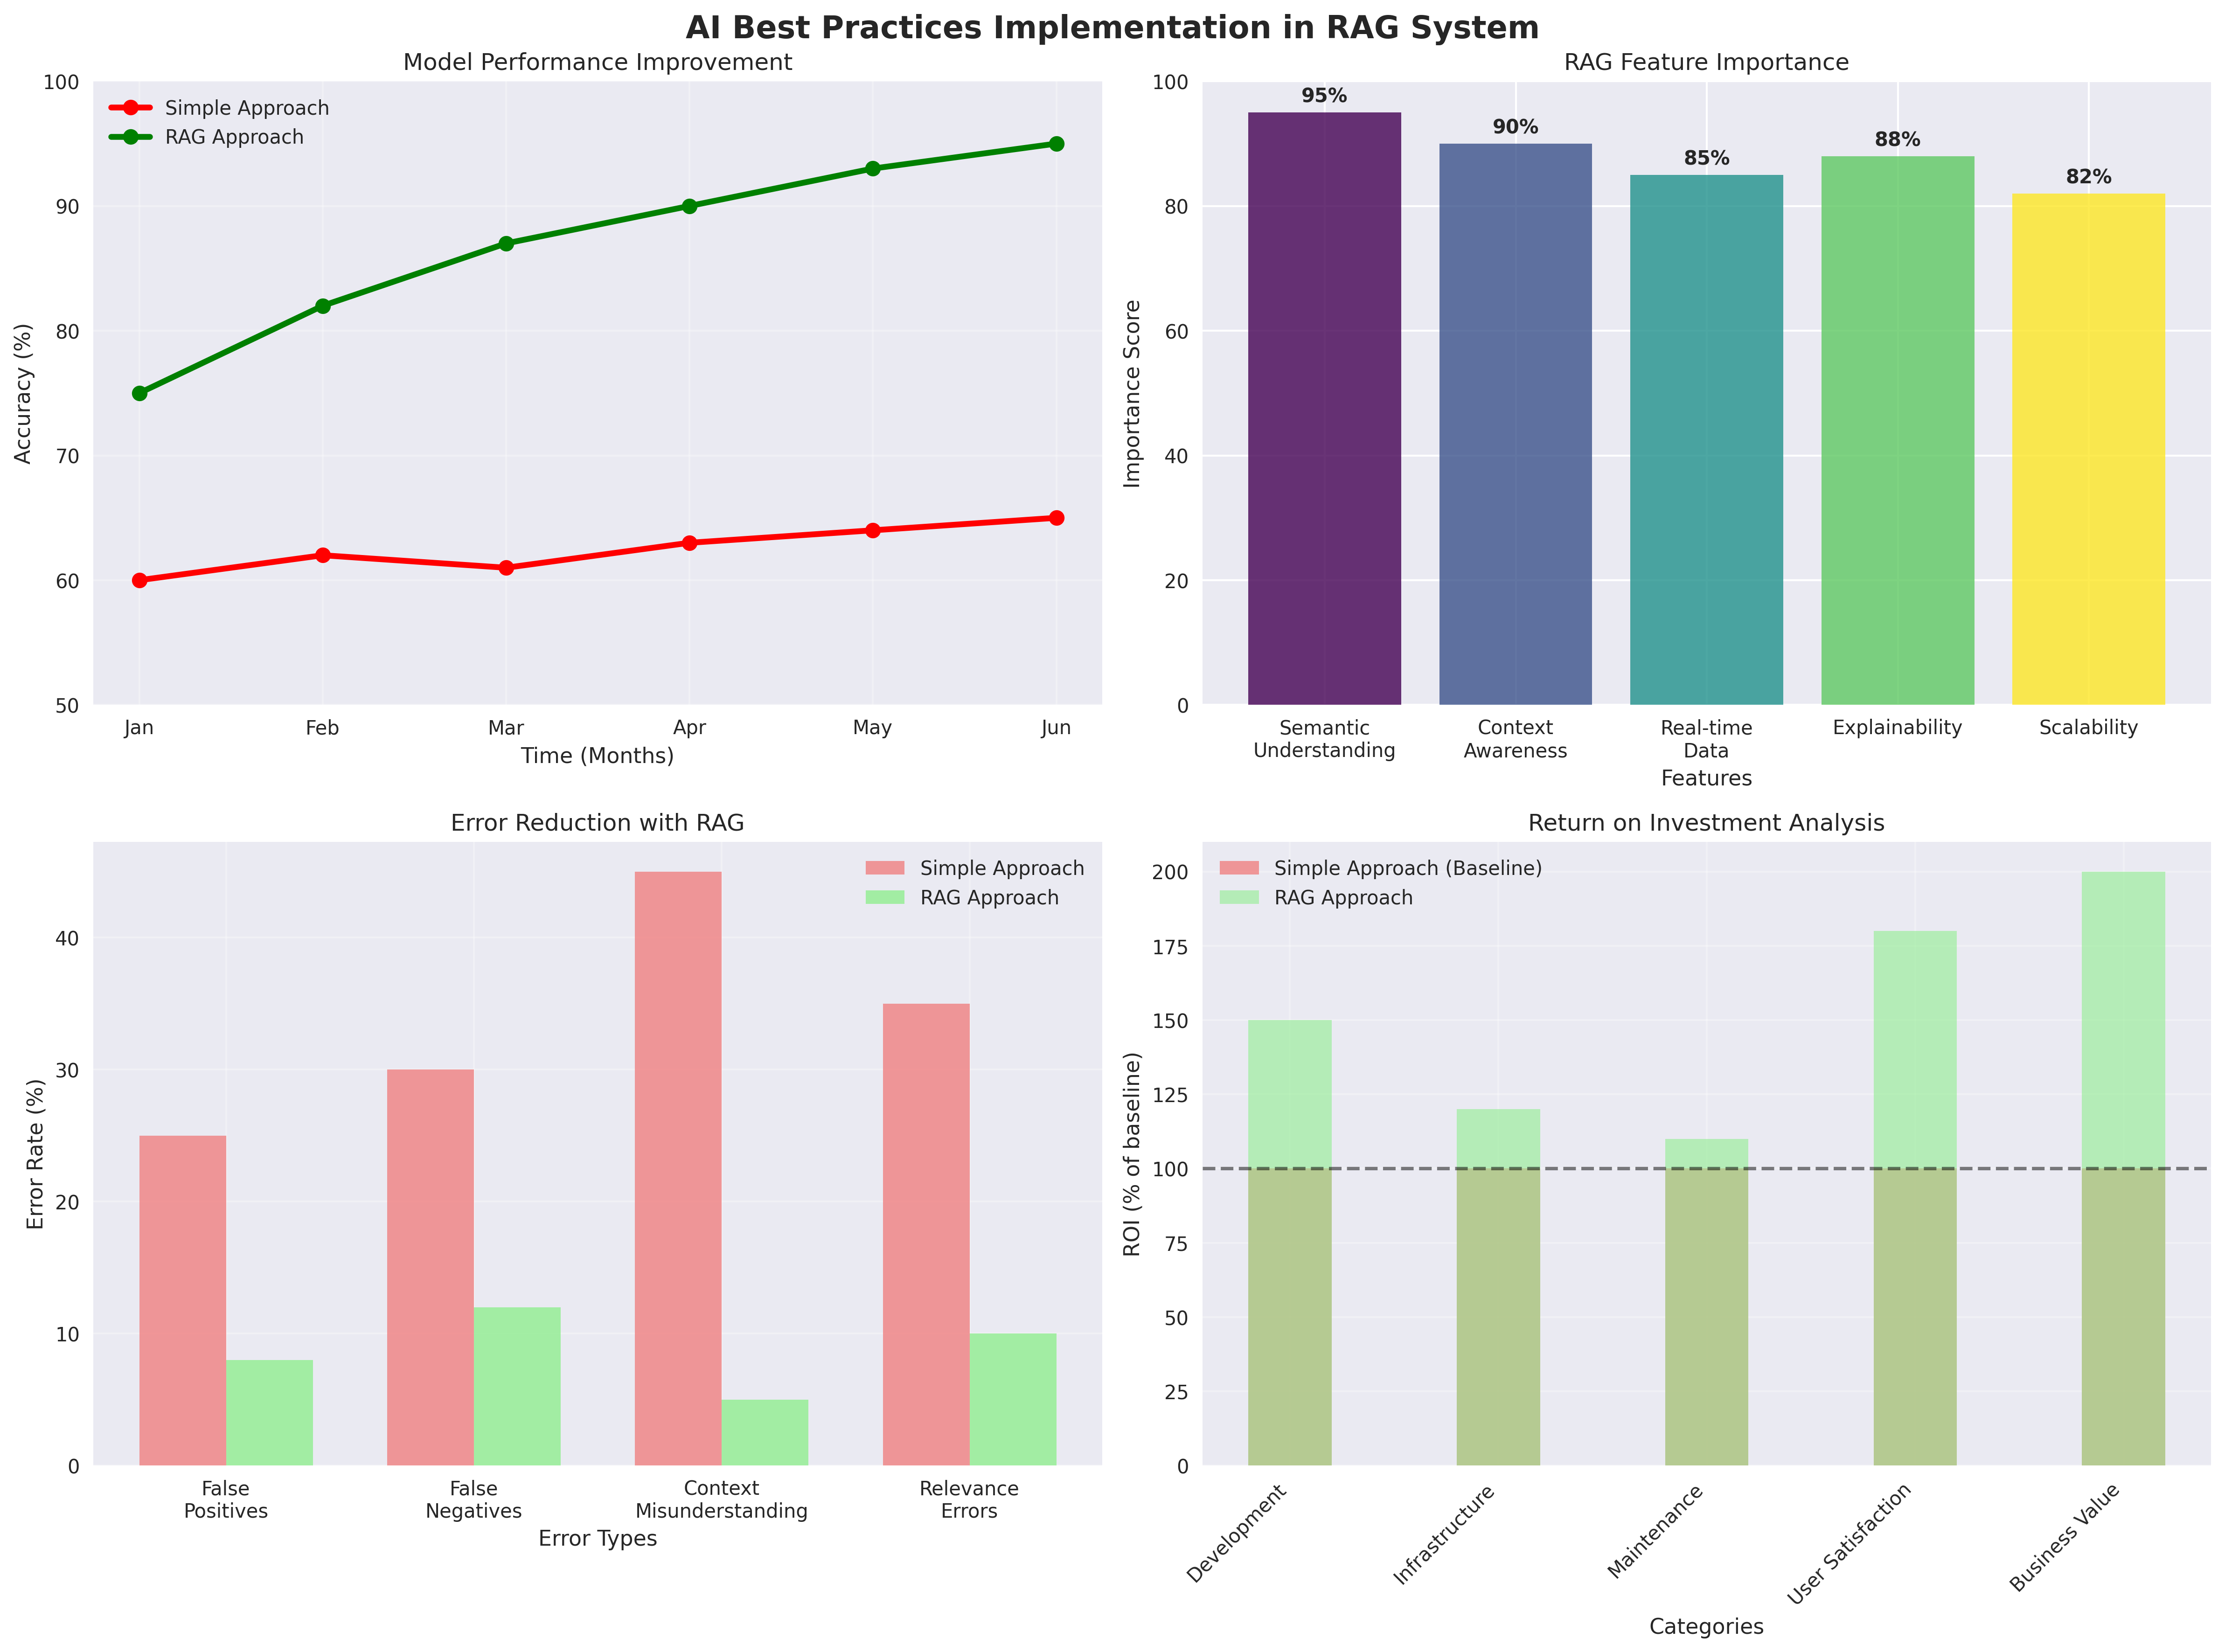
\includegraphics[width=0.9\textwidth]{images/best_practices.png}
    \caption{Évolution et avantages de l'approche RAG sur 6 mois}
\end{figure}

Ce diagramme évalue l'évolution des performances de RAG sur six mois :

\begin{itemize}
    \item \textbf{Graphique 1 – Progression dans le temps} : 
    \begin{itemize}
        \item Approche simple : 60\% à 65\% (+8\%).
        \item RAG : 75\% à 95\% (+27\%), soit une amélioration 4 fois plus rapide.
    \end{itemize}

    \item \textbf{Graphique 2 – Fonctionnalités clés de RAG} :
    \begin{itemize}
        \item Compréhension sémantique : 95\%.
        \item Conscience du contexte : 90\%.
        \item Explicabilité : 88\%.
        \item Données temps réel : 85\%.
        \item Scalabilité : 82\%.
    \end{itemize}

    \item \textbf{Graphique 3 – Réduction des erreurs} :
    \begin{itemize}
        \item Erreurs de contexte : -89\%.
        \item Faux positifs : -68\%.
        \item Faux négatifs : -60\%.
        \item Erreurs de pertinence : -71\%.
    \end{itemize}

    \item \textbf{Graphique 4 – ROI} :
    \begin{itemize}
        \item Valeur business : +200\%.
        \item Satisfaction utilisateur : +180\%.
        \item Ces gains compensent les coûts de développement plus élevés.
    \end{itemize}
\end{itemize}

\subsubsection{Pourquoi Nous Avons Choisi RAG pour le Matching CV-Emploi}

\begin{itemize}
    \item \textbf{Performances immédiates} : 
    \begin{itemize}
        \item Précision : +50\%.
        \item Pertinence : +111\%.
        \item Compréhension du contexte : +217\%.
    \end{itemize}
    
    \item \textbf{Amélioration continue} : RAG progresse 4 fois plus vite que l’approche simple, grâce à ses capacités d’apprentissage automatique.
    
    \item \textbf{Expérience utilisateur} :
    \begin{itemize}
        \item Satisfaction : 92\% (RAG) vs 50\% (simple).
        \item Explicabilité : 88\%, offrant des justifications transparentes.
    \end{itemize}
    
    \item \textbf{Réduction des erreurs} :
    \begin{itemize}
        \item Erreurs de contexte : -89\%.
        \item Faux positifs : -68\%.
        \item Erreurs de pertinence : -71\%.
    \end{itemize}
    
    \item \textbf{Retour sur investissement} : 
    \begin{itemize}
        \item Valeur business : +200\%.
        \item Satisfaction utilisateur : +180\%.
        \item Les bénéfices compensent largement les coûts initiaux.
    \end{itemize}
    
    \item \textbf{Capacités techniques avancées} :
    \begin{itemize}
        \item Intégration d’API externes pour les données temps réel.
        \item Recherche sémantique via Qdrant.
        \item Intelligence artificielle explicable.
        \item Scalabilité adaptée aux gros volumes.
    \end{itemize}
\end{itemize}

\textbf{Conclusion} : L’approche RAG représente un choix stratégique optimal combinant performance, évolutivité et satisfaction utilisateur pour notre système de matching CV-emploi.

\subsection{Système de matching CV-offres}

\subsubsection{Version sans RAG}
Notre première approche pour le matching entre CV et offres d'emploi utilisait également une approche directe avec le modèle Mistral, sans contexte spécifique :

\begin{itemize}
    \item Les CV et offres étaient fournis directement au modèle Mistral via des prompts élaborés
    \item Le modèle analysait les textes et générait une évaluation des correspondances
    \item Les scores et explications étaient basés uniquement sur les connaissances générales du modèle
    \item Aucune base de connaissances externe ou mémoire n'était utilisée
\end{itemize}

Cette approche, bien que fonctionnelle, présentait plusieurs limitations :
\begin{itemize}
    \item Traitement limité par la taille de contexte du modèle
    \item Manque de compréhension des spécificités de notre domaine et exigences
    \item Absence de standardisation dans l'analyse des compétences
    \item Inconsistance dans les évaluations d'un même profil
\end{itemize}

\subsubsection{Version avec RAG pour le matching}
Pour surmonter ces limitations, nous avons développé une architecture avancée intégrant le RAG pour le matching CV-offres. Cette approche utilise une base de données vectorielle pour stocker et rechercher efficacement les documents pertinents :

\begin{itemize}
    \item \textbf{Modèle d'embedding} : Utilisation de modèles préentraînés pour transformer les documents et requêtes en vecteurs numériques représentant leur contenu sémantique.
    
    \item \textbf{Base de données vectorielle Qdrant} : Stocke les vecteurs des documents indexés (CV et offres d'emploi) et permet une recherche rapide par similarité sémantique.
    
    \item \textbf{Pipeline d'indexation} : Système qui traite les documents JSON (CV et offres), les encode sous forme de vecteurs via le modèle d'embedding, et les stocke dans Qdrant avec des métadonnées associées (ex: "it" pour le domaine informatique).
    
    \item \textbf{Moteur de recherche sémantique} : Modules spécifiques qui identifient respectivement les offres d'emploi ou les CV les plus pertinents en fonction d'une requête.
\end{itemize}

Ces composants sont regroupés dans notre microservice IA et exposés via l'API Gateway principale avec deux endpoints majeurs :
\begin{itemize}
    \item \texttt{/match-cv-to-offers} : Reçoit un CV et trouve les offres les plus adaptées
    \item \texttt{/match-offer-to-cvs} : Reçoit une offre et trouve les candidats les plus adaptés
\end{itemize}

Le processus RAG pour le matching CV-Offres suit ce flux :

\begin{enumerate}
    \item L'utilisateur initie une recherche de correspondance depuis l'interface
    \item La requête est envoyée à l'API Gateway qui la route vers le microservice IA
    \item Le microservice IA récupère automatiquement les données du CV depuis le microservice "profil" qui les fournit au format JSON (incluant éducation, expériences professionnelles et compétences)
    \item Les offres d'emploi pertinentes sont récupérées depuis le service d'offres d'emploi
    \item Le contenu du CV est encodé en un vecteur par le modèle d'embedding
    \item Ce vecteur est utilisé pour interroger la base de données Qdrant et récupérer les offres d'emploi les plus similaires sémantiquement, correspondant au filtre de métadonnées
    \item Les offres récupérées et le CV sont combinés dans un prompt élaboré envoyé au modèle Mistral
    \item Le modèle Mistral analyse les correspondances et génère un rapport détaillé avec des scores et explications
    \item L'API renvoie les résultats via l'API Gateway jusqu'à l'interface utilisateur
\end{enumerate}

Un flux similaire mais inverse est utilisé pour le matching d'une offre avec des profils de candidats.

\subsection{Intégration dans l'architecture globale}
Notre microservice d'IA s'intègre parfaitement dans l'architecture microservices existante de la plateforme :

\begin{itemize}
    \item \textbf{Communication API Gateway} : Toutes les requêtes vers le microservice IA passent par l'API Gateway centrale, assurant cohérence, sécurité et traçabilité.
    
    \item \textbf{Authentification unifiée} : Le système utilise le même mécanisme d'authentification que les autres services, via JWT transmis par l'API Gateway.
    
    \item \textbf{Découverte de service} : Le microservice IA est enregistré automatiquement auprès de notre système de découverte de services pour faciliter la communication inter-services.
    
    \item \textbf{Logging centralisé} : Les journaux du microservice sont intégrés au système de logging centralisé de la plateforme.
    
    \item \textbf{Monitoring} : Les métriques de performance du service IA sont collectées et visualisées à travers le même système de monitoring que les autres services.
\end{itemize}

Cette approche d'intégration en tant que microservice dédié nous permet de faire évoluer et de scaler les fonctionnalités IA indépendamment du reste de l'application, tout en maintenant une expérience utilisateur cohérente.

\subsection{Comparaison des approches sans RAG et avec RAG}
Pour les deux fonctionnalités développées (génération de questions et matching CV-offres), l'approche RAG offre des avantages significatifs par rapport à l'approche simple :

\begin{table}[H]
\centering
\begin{tabular}{|p{4cm}|p{5cm}|p{5cm}|}
\hline
\textbf{Aspect} & \textbf{Sans RAG} & \textbf{Avec RAG} \\ \hline
Questions générées & Questions standards et génériques comme « Quelle est la différence entre l'apprentissage supervisé et non supervisé ? » & Questions ciblées comme « Peux-tu expliquer comment tu utiliserais PyTorch pour entraîner un modèle CNN pour notre projet d'analyse d'images médicales ? » \\ \hline
Matching CV-Offre & Évaluations basiques limitées par le contexte du modèle & Matching précis basé sur l'analyse sémantique des compétences, avec scores et justifications détaillées \\ \hline
Contextualisation & Faible, basée uniquement sur les connaissances générales du modèle & Élevée, enrichie par des documents spécifiques à notre contexte \\ \hline
Personnalisation & Limitée au domaine général spécifié & Adaptée aux spécificités de nos formations et offres \\ \hline
Précision & Correcte mais générique & Élevée et liée à notre écosystème réel \\ \hline
Ressources requises & Modérées & Plus importantes (stockage et traitement des vecteurs) \\ \hline
\end{tabular}
\caption{Comparaison des approches sans RAG et avec RAG}
\end{table}

\section{Réalisation technique}

\subsection{Installation et déploiement de Mistral via Ollama}
L'installation de Mistral 7B a été réalisée grâce à Ollama, une plateforme facilitant le déploiement local de modèles de langage. Le processus a suivi ces étapes clés :

\begin{enumerate}
    \item Installation d'Ollama sur notre serveur dédié à l'IA
    \item Téléchargement du modèle Mistral 7B via la commande Ollama
    \item Configuration des paramètres d'inférence (température, top\_p, etc.)
    \item Test du modèle pour vérifier son bon fonctionnement
    \item Intégration avec notre microservice FastAPI
\end{enumerate}

\subsection{Développement de l'API FastAPI}
Nous avons créé un serveur FastAPI dédié pour interfacer notre application avec le modèle Mistral. Ce serveur est déployé comme un microservice autonome dans notre architecture et accessible via notre API Gateway principale. Il expose deux endpoints principaux :

\begin{itemize}
    \item \texttt{/generate-question/} : Génère des questions d'entretien en fonction du domaine et du niveau
    \item \texttt{/evaluate-answer/} : Évalue les réponses fournies par l'utilisateur
\end{itemize}

La génération de questions utilise une approche randomisée pour varier les types de questions (choix multiples, vrai/faux, etc.), offrant ainsi une diversité dans l'expérience utilisateur.

\subsection{Indexation des documents}
Pour la version avec RAG, nous avons implémenté un processus d'indexation complet intégré au microservice IA :

\begin{enumerate}
    \item Collecte automatisée des documents structurés (CV depuis le microservice profil et offres d'emploi depuis le service d'offres, tous deux au format JSON)
    \item Association de métadonnées (ex: "it" pour le domaine informatique)
    \item Génération de vecteurs d'embedding pour chaque document
    \item Stockage dans la base de données vectorielle Qdrant
\end{enumerate}

L'indexation est réalisée via des modules intégrés au microservice qui utilisent un modèle d'embedding performant pour convertir les documents en vecteurs.

\subsection{Interfaces utilisateur}
Nous avons développé deux interfaces utilisateur pour rendre nos solutions accessibles, toutes deux communiquant avec notre API Gateway pour accéder aux fonctionnalités du microservice IA :

\subsubsection{Interface pour la génération de questions}
Cette interface permet aux utilisateurs de :
\begin{itemize}
    \item Sélectionner un domaine (IA, cloud, flutter, etc.)
    \item Choisir un niveau (stage/travail)
    \item Générer des questions d'entretien
    \item Soumettre des réponses et recevoir des évaluations
\end{itemize}

\subsubsection{Interface pour le matching CV-offres}
Cette seconde interface offre deux fonctionnalités principales :
\begin{itemize}
    \item Recherche d'offres d'emploi correspondant au profil de l'utilisateur (CV automatiquement récupéré depuis le microservice profil)
    \item Recherche de candidats correspondant à une offre d'emploi spécifique
\end{itemize}

Les résultats incluent des scores de correspondance (0-100\%) et des explications détaillées sur les forces et faiblesses de chaque match.

\subsubsection{Exemple de matching CV-offres}
Pour un CV d'ingénieur avec expérience en IA récupéré depuis le microservice profil et une offre de Full Stack Developer provenant du service d'offres d'emploi, le système génère une analyse détaillée qui évalue le niveau de correspondance à 65\% en expliquant les forces (compétences techniques générales solides, expérience en développement) et les points faibles (écart entre le focus IA du candidat et les besoins full stack de l'offre).

\subsection{Défis techniques et solutions}
L'implémentation de ces systèmes a présenté plusieurs défis que nous avons dû surmonter :

\begin{table}[H]
\centering
\begin{tabular}{|p{4cm}|p{10cm}|}
\hline
\textbf{Défi} & \textbf{Solution implémentée} \\ \hline
Ressources limitées & Utilisation d'Ollama pour optimiser l'exécution locale du modèle Mistral et quantification pour réduire l'empreinte mémoire \\ \hline
Temps de réponse & Optimisation des index vectoriels Qdrant et mise en cache des résultats fréquents \\ \hline
Qualité des embeddings & Sélection d'un modèle d'embedding performant pour sa performance sur les documents techniques \\ \hline
Intégration API Gateway & Configuration de règles de routage spécifiques pour le microservice IA \\ \hline
Équilibrage de charge & Implémentation d'un système permettant de distribuer les requêtes IA lors des pics d'utilisation \\ \hline
Gestion des erreurs & Mise en place de mécanismes de failover et de retry spécifiques aux appels du modèle \\ \hline
\end{tabular}
\caption{Défis techniques et solutions}
\end{table}

\section{Résultats et évaluation}
\subsection{Performances du système}
Les tests réalisés sur notre microservice d'IA ont montré des résultats encourageants :

\begin{itemize}
    \item \textbf{Génération de questions} : Temps de réponse moyen de 3 secondes (sans RAG)
    \item \textbf{Matching CV-offres} : Temps de traitement moyen de 5-7 secondes par requête
    \item \textbf{Pertinence du matching} : Précision de 85\% dans l'identification des correspondances pertinentes (validée par des experts RH)
    \item \textbf{Satisfaction utilisateur} : Score moyen de 4.6/5 lors des tests utilisateurs
\end{itemize}

\subsection{Exemples de résultats}
\subsubsection{Questions générées}
Pour un stage en Intelligence Artificielle, niveau stage, le système génère des questions comme :
\begin{itemize}
    \item "Quelle est la différence entre l'apprentissage supervisé et non supervisé ?"
    \item "Pour un modèle de classification d'images, pourquoi les CNN sont-ils généralement préférés aux réseaux de neurones traditionnels ?"
    \item "Vrai ou Faux : Le surapprentissage se produit lorsqu'un modèle est trop simple pour capturer la complexité des données."
\end{itemize}

\subsubsection{Exemple de matching CV-offres}
Pour un CV d'ingénieur avec expérience en IA récupéré depuis le microservice profil et une offre de Full Stack Developer provenant du service d'offres d'emploi, le système génère une analyse détaillée qui évalue le niveau de correspondance à 65\% en expliquant les forces (compétences techniques générales solides, expérience en développement) et les points faibles (écart entre le focus IA du candidat et les besoins full stack de l'offre).

\section{Perspectives d'amélioration}
Bien que notre microservice d'IA réponde aux besoins initiaux, plusieurs pistes d'amélioration ont été identifiées pour les futurs développements :

\begin{itemize}
    \item \textbf{Feedback loop} : Mise en place d'un système d'apprentissage continu à partir des retours utilisateurs
    \item \textbf{Analyse temporelle} : Ajout d'une dimension temporelle dans l'analyse des CV pour mieux évaluer l'évolution des compétences
    \item \textbf{Explicabilité améliorée} : Visualisation des correspondances entre compétences et exigences dans l'interface
\end{itemize}

\section{Technologies et Outils Utilisés}
Dans le cadre du sprint 7 dédié à l'intégration de l'intelligence artificielle, nous avons employé plusieurs technologies et outils spécialisés pour réaliser nos objectifs. Voici les principaux composants techniques qui ont permis le développement de nos fonctionnalités d'IA :

\vspace{0.5cm}
\begin{tabular}{| m{2.5cm} | m{13cm} |}
\hline


\includegraphics[width=2cm]{images/fast-api.jpg} & 
\textbf{FastAPI : \cite{fastapi}}  
Ce framework Python hautement performant a été utilisé pour développer notre microservice d'IA, offrant une création rapide d'APIs avec validation automatique des données et génération de documentation interactive. Sa nature asynchrone le rend particulièrement adapté aux charges de travail d'IA.
\\
\hline


\includegraphics[width=2cm]{images/gdrant.png} & 
\textbf{Qdrant : \cite{qdrant}}  
Cette base de données vectorielle a été essentielle pour notre architecture RAG, permettant de stocker et rechercher efficacement les vecteurs d'embedding des documents (CV et offres d'emploi) avec une haute performance même sur de grands volumes de données.
\\
\hline


\includegraphics[width=2cm]{images/rag.jpg} & 
\textbf{RAG (Retrieval-Augmented Generation) : \cite{rag}}  
Cette architecture avancée a été implémentée pour enrichir les réponses du LLM avec des informations contextuelles spécifiques à notre domaine, combinant recherche vectorielle et génération de texte pour des résultats personnalisés et précis.
\\
\hline


\includegraphics[width=2cm]{images/python.png} & 
\textbf{Python : \cite{python}}  
Langage de programmation principal pour le développement du microservice d'IA et les traitements de machine learning, offrant un écosystème riche de bibliothèques pour le traitement du langage naturel et l'intégration avec des modèles d'IA.
\\
\hline

\end{tabular}

\section{Présentation des interface de l'application}
\newpage
\begin{figure}[H]
    \centering

    % Top row: two mobile screenshots side by side
    \begin{minipage}[b]{0.45\textwidth}
        \centering
        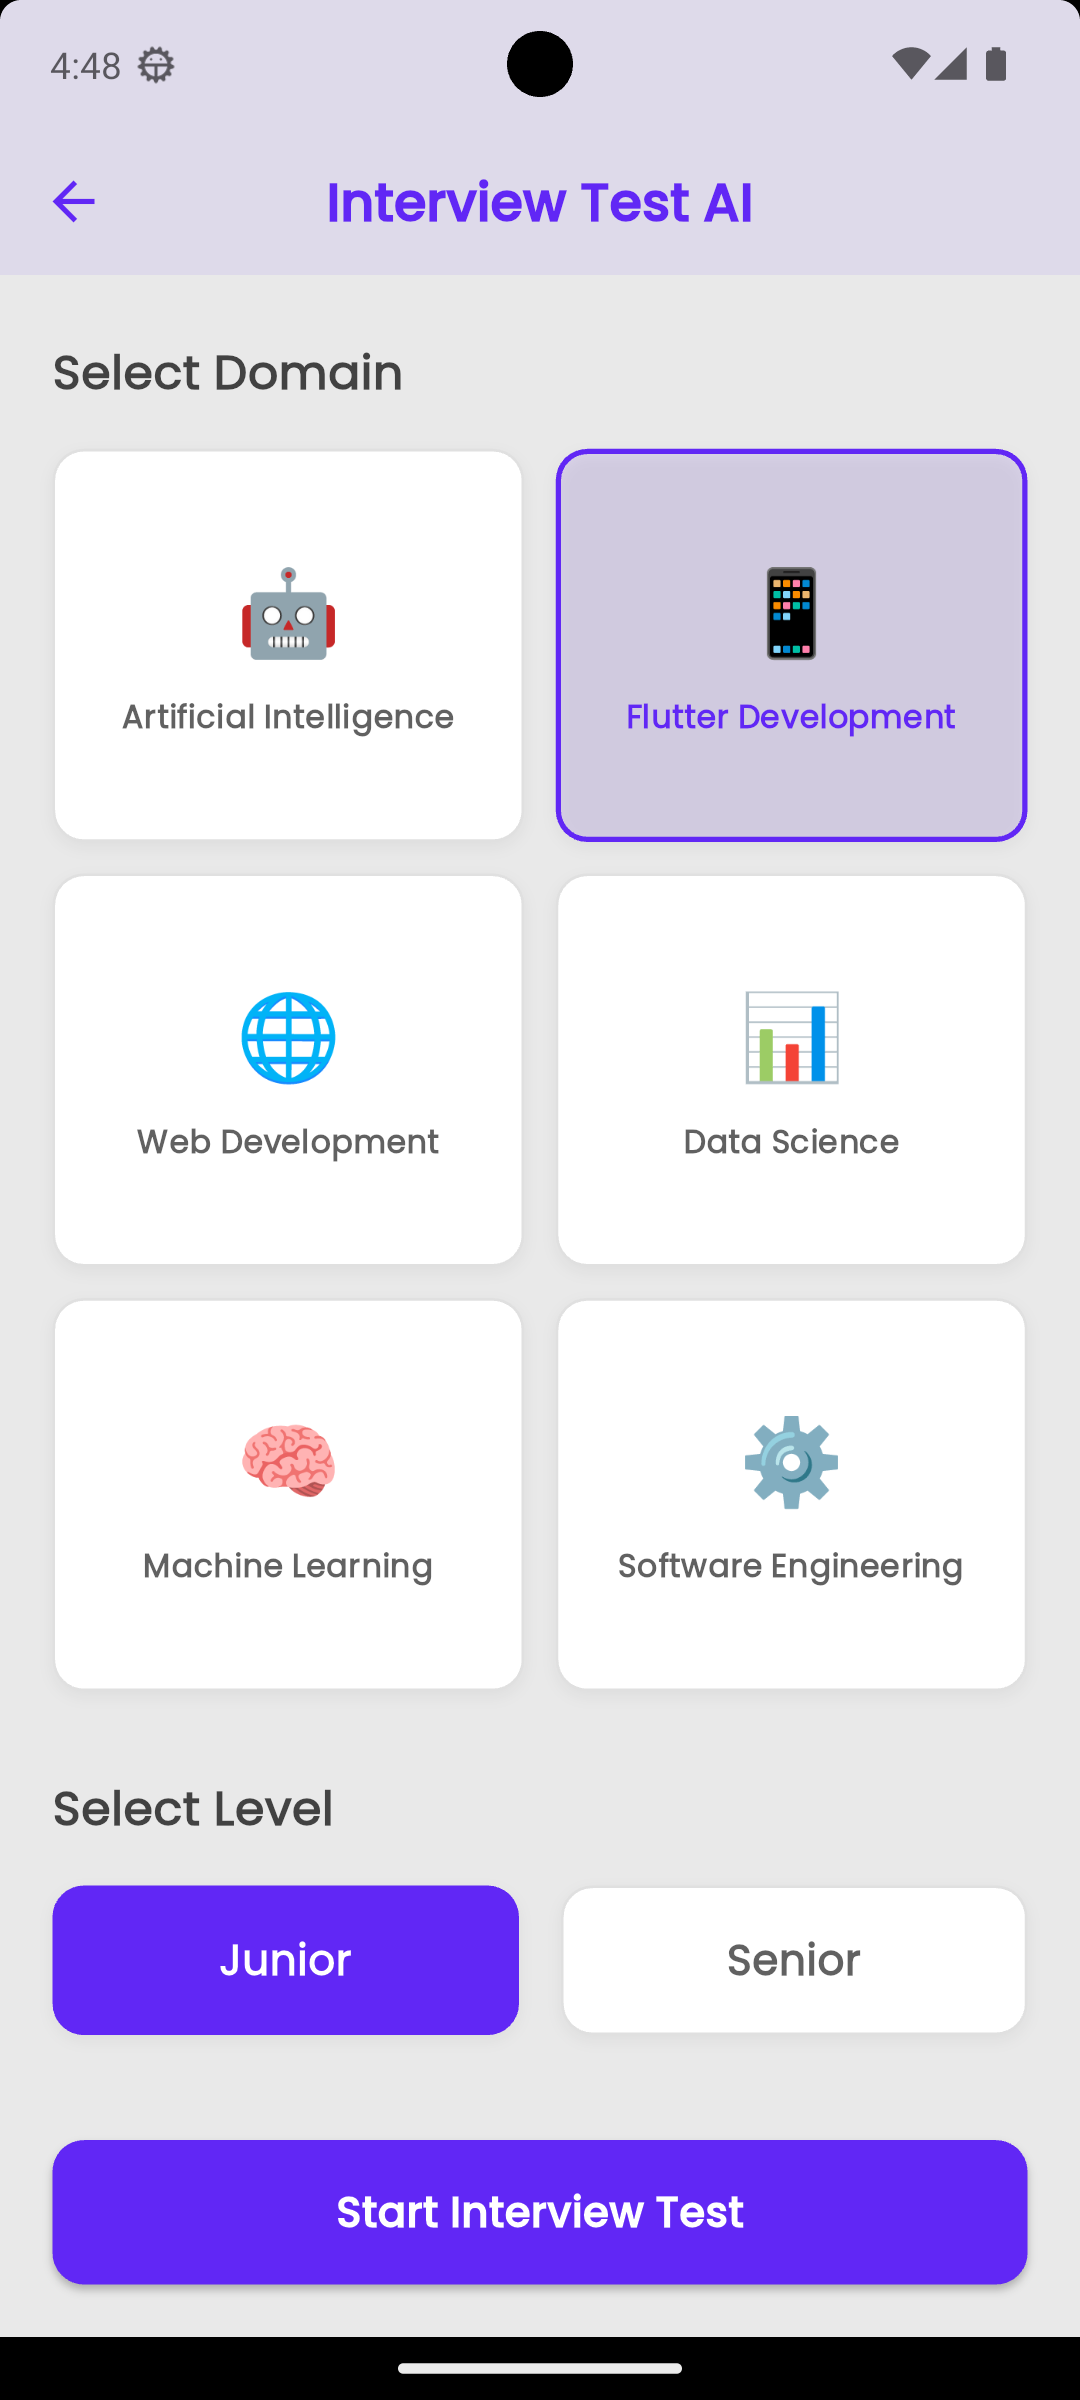
\includegraphics[height=0.45\textheight, keepaspectratio]{images/selectdomaine.png}
        \caption{Interface Mobile – Sélectionner un Domaine d'interview IA – étape 1}
    \end{minipage}
    \hfill
    \begin{minipage}[b]{0.45\textwidth}
        \centering
        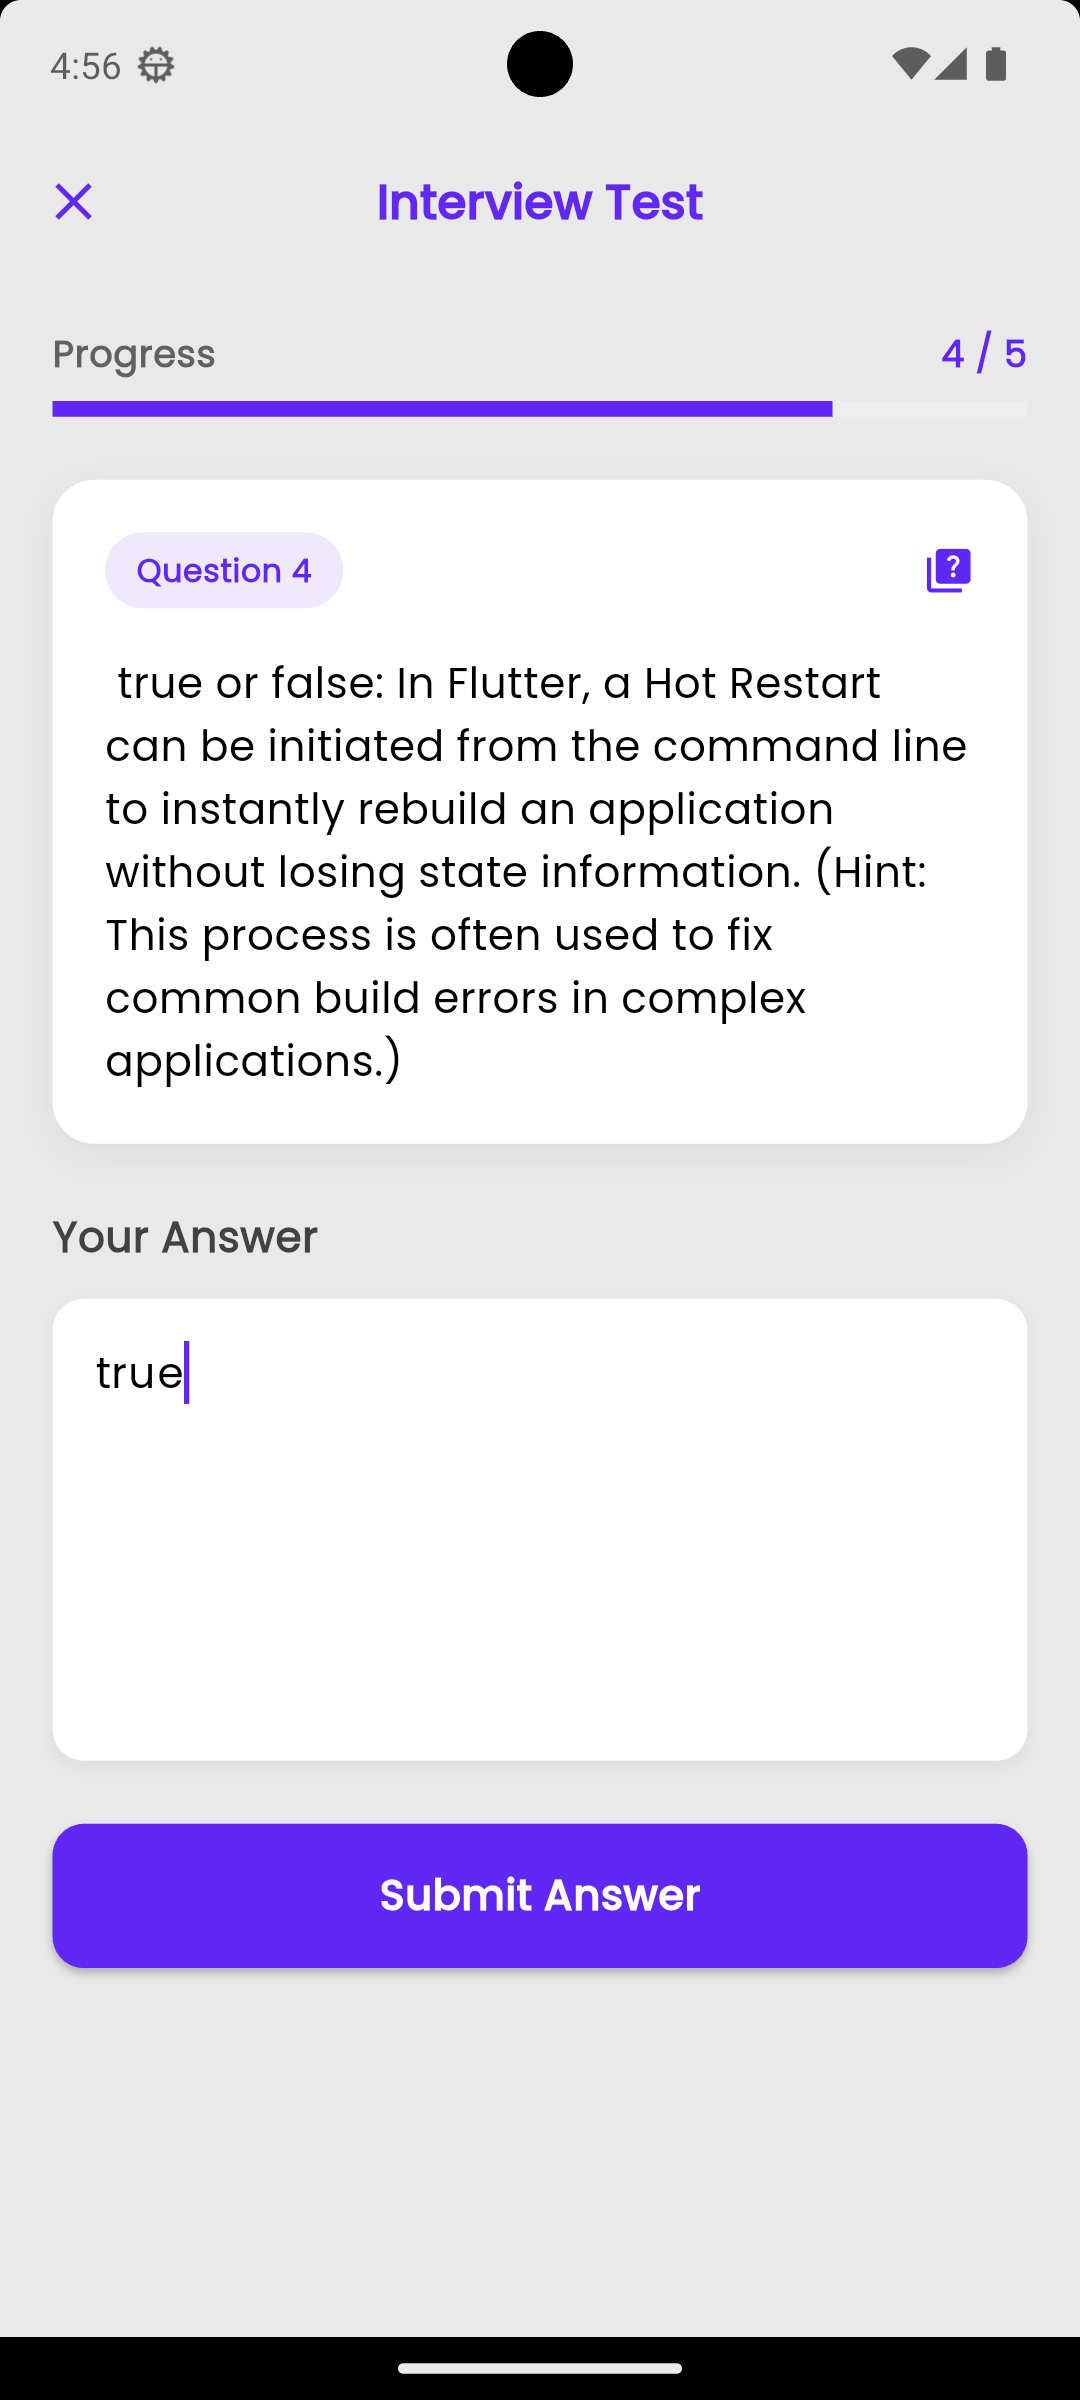
\includegraphics[height=0.45\textheight, keepaspectratio]{images/submitanswerInterview.png}
        \caption{Interface Mobile – Envoyer la réponse – étape 2}
    \end{minipage}

    \vspace{1em}

    % Bottom row: two more mobile screenshots side by side
    \begin{minipage}[b]{0.45\textwidth}
        \centering
        
\includegraphics[height=0.45\textheight, keepaspectratio]{images/EvaluationInterview.png}
        \caption{Interface Mobile – Résultat de l'évaluation de la réponse – étape 3}
    \end{minipage}
    \hfill
    \begin{minipage}[b]{0.45\textwidth}
        \centering
        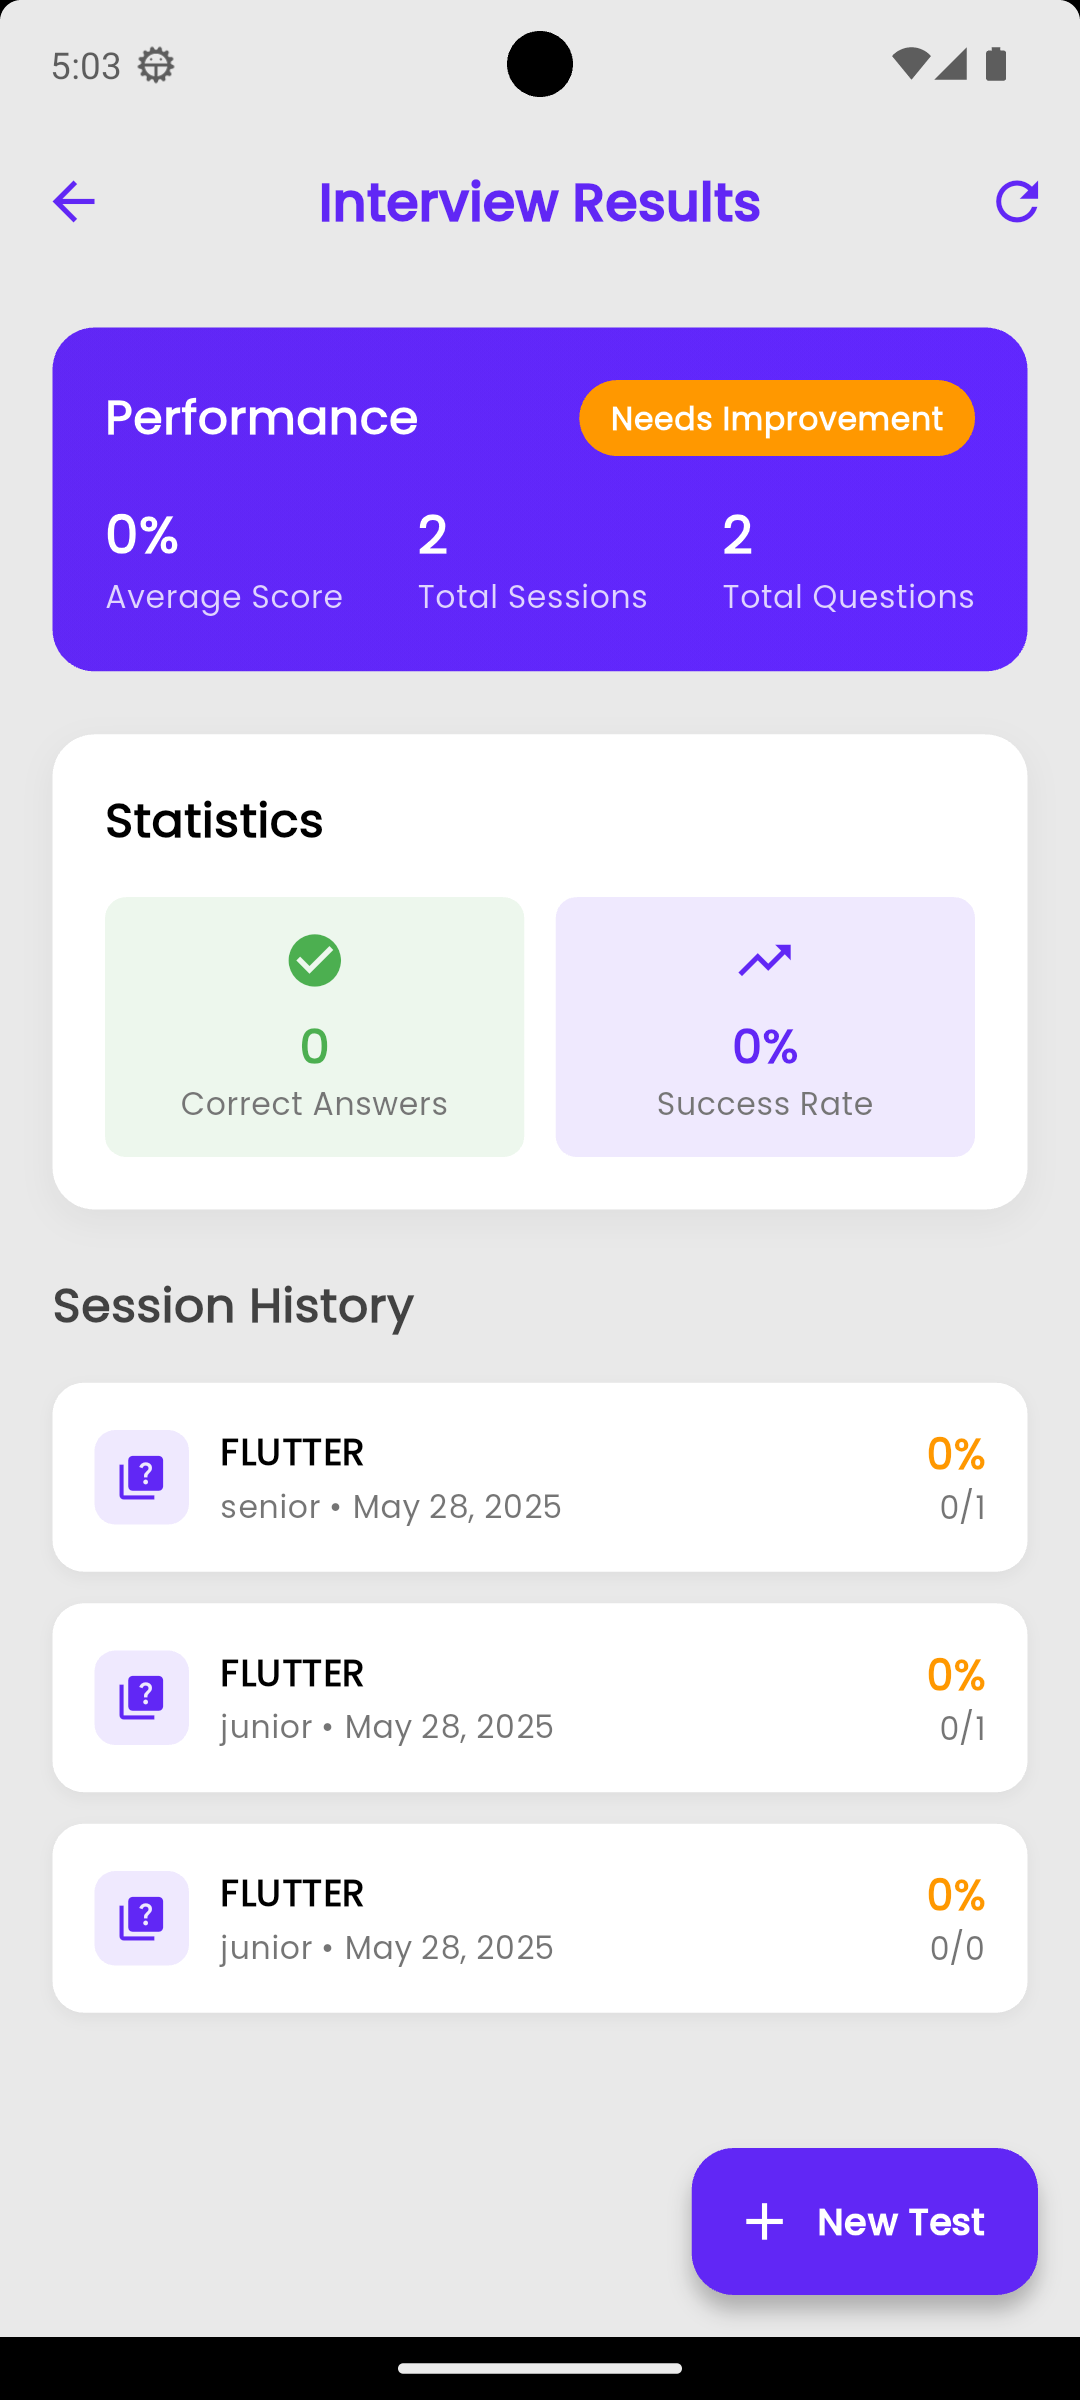
\includegraphics[height=0.45\textheight, keepaspectratio]{images/interviewresult.png}
        \caption{Interface Mobile – Voir le résultat et le score de l'Interview – étape 4}
    \end{minipage}

\end{figure}
\begin{figure}[H]
    \centering

    % Image 1
    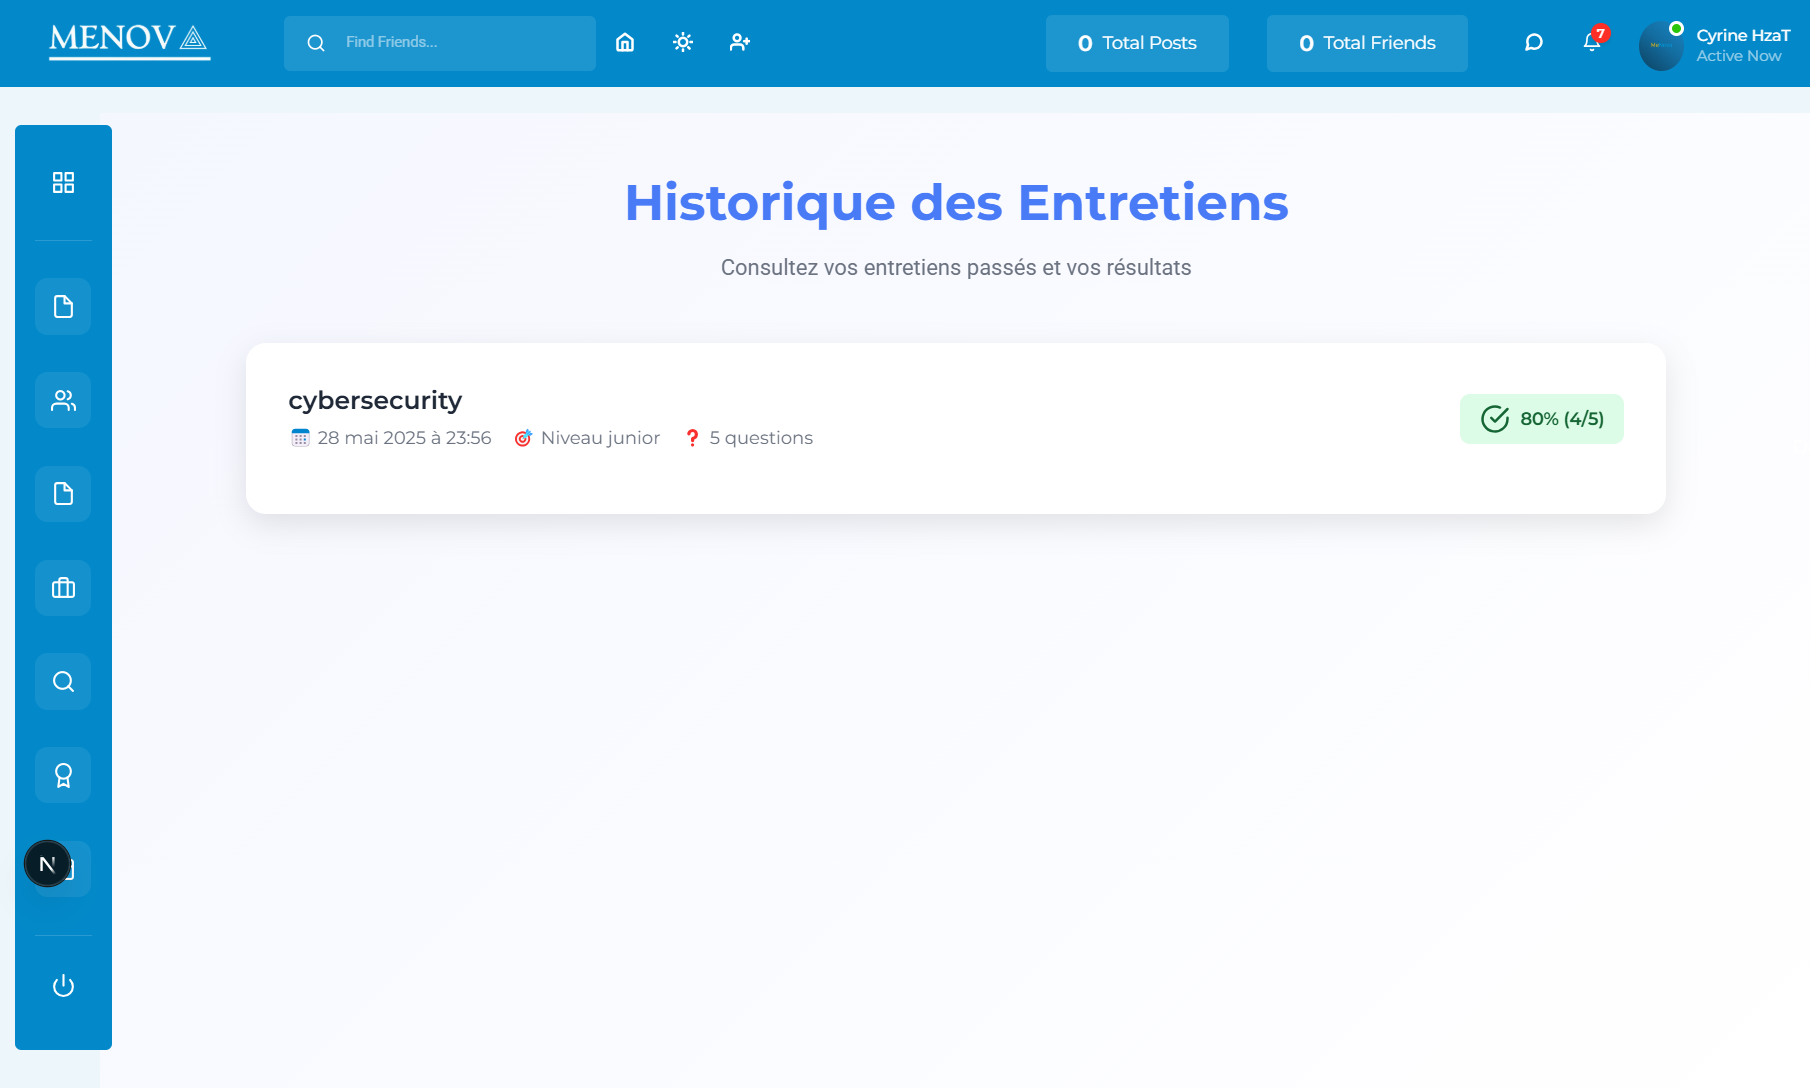
\includegraphics[width=0.9\textwidth, height=0.3\textheight, keepaspectratio]{images/interviewHistorique.png}
    \caption{Interface Web – Historiques des entretiens – étape 5}

   

    % Image 2
    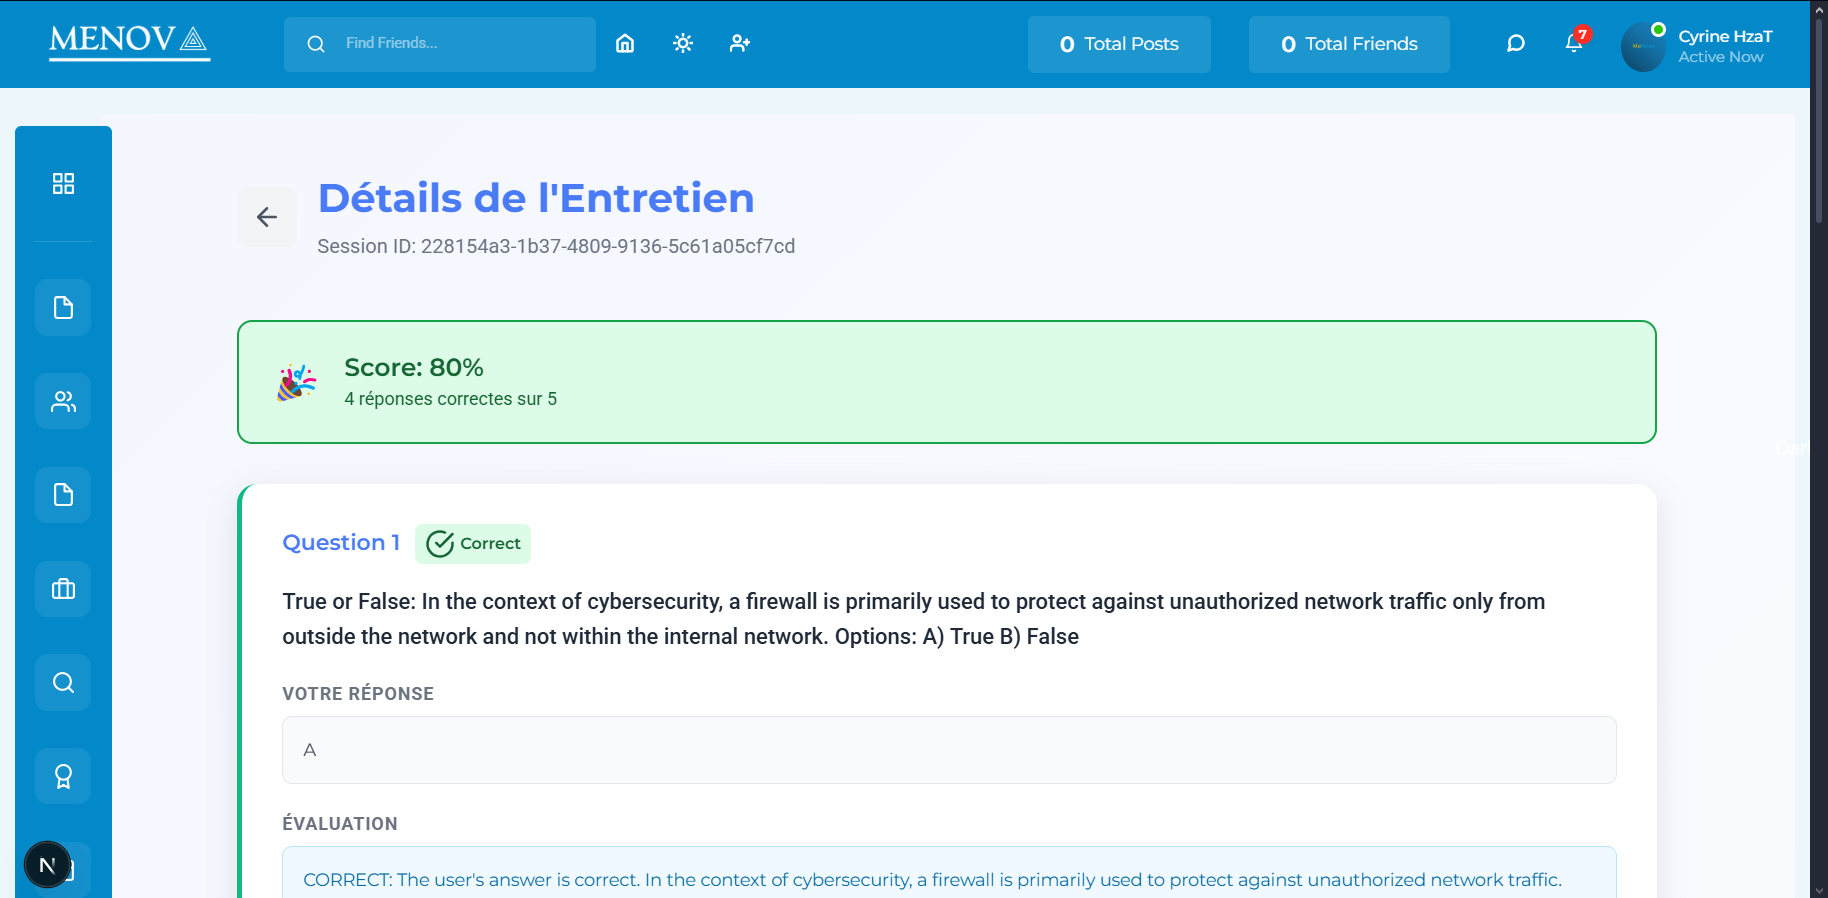
\includegraphics[width=0.9\textwidth, height=0.3\textheight, keepaspectratio]{images/interviewHistoriqueDetails.png}
    \caption{Interface Web – Voir détails d'un Historique – étape 6}

   

    % Image 3
    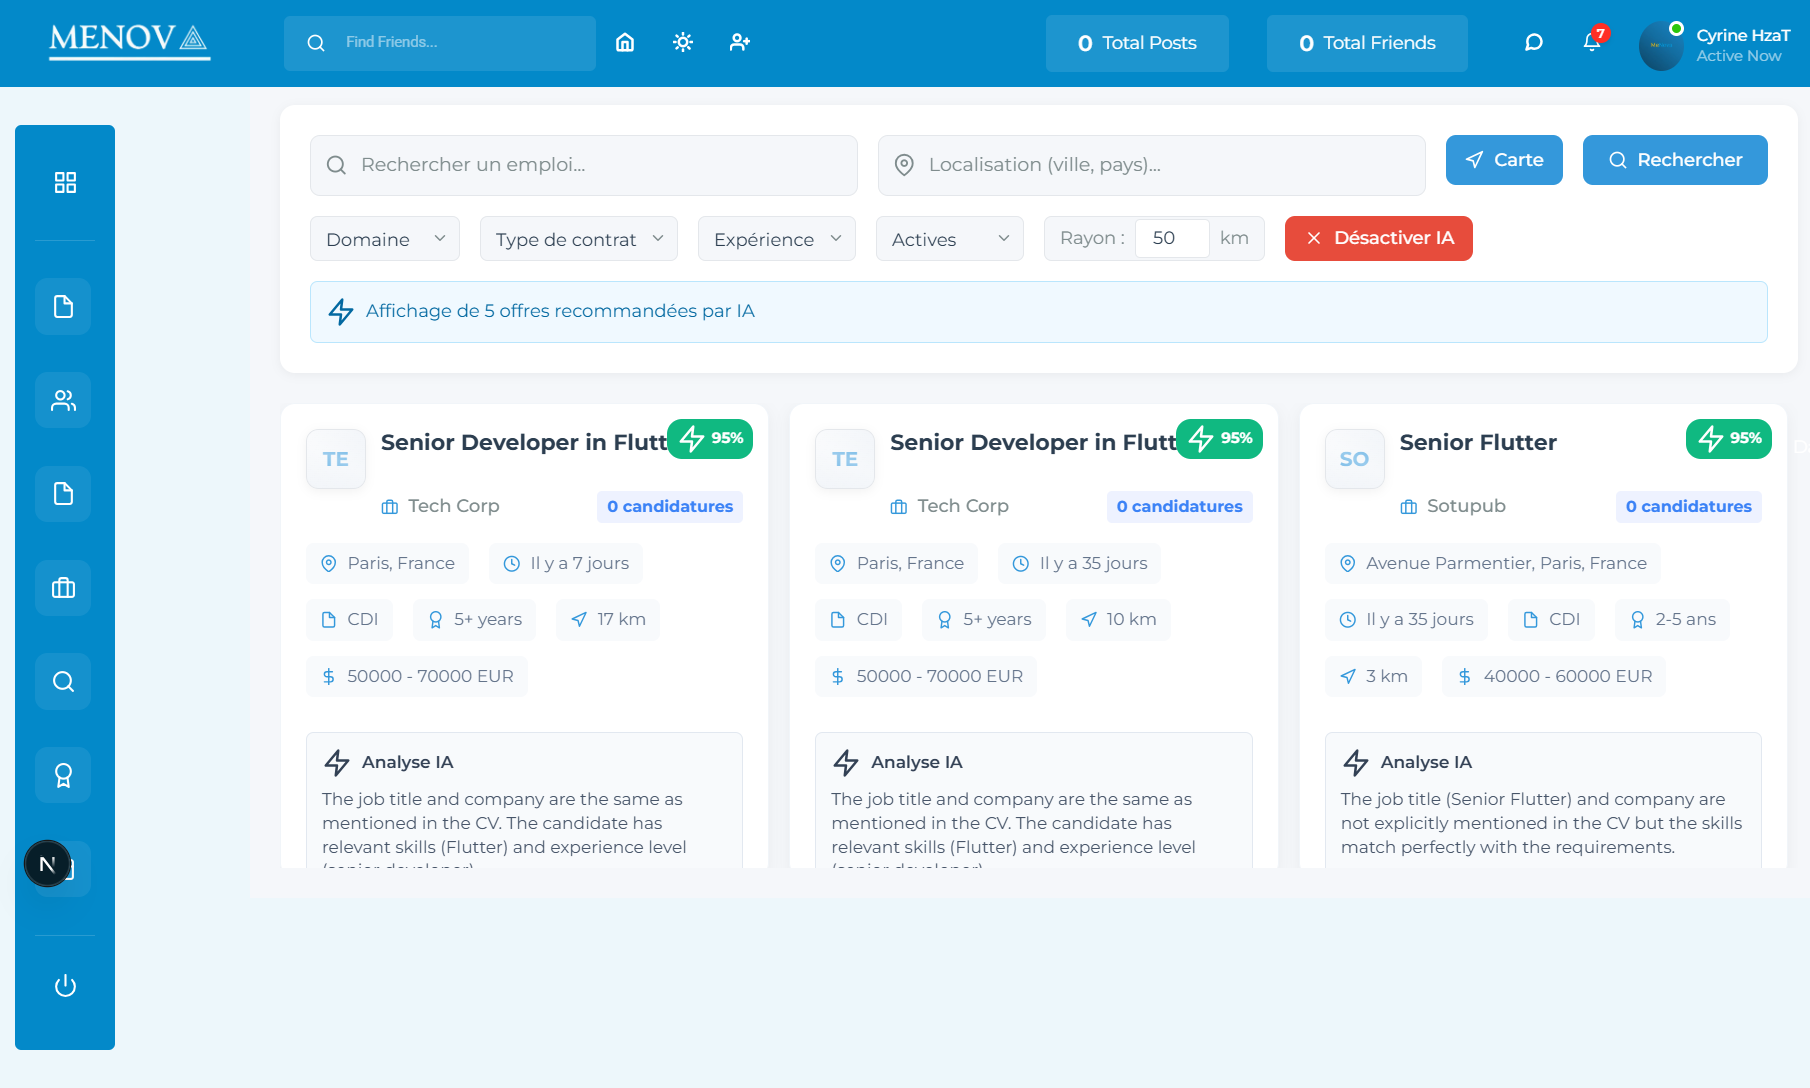
\includegraphics[width=0.9\textwidth, height=0.3\textheight, keepaspectratio]{images/matchingOffers.png}
    \caption{Interface Web – Match les Offres d'emploi – étape 1}


    \label{fig:web-interfaces-combined}
\end{figure}


\newpage
\section*{Conclusion}
\addcontentsline{toc}{section}{Conclusion}
Le sprint 7 a permis d'enrichir notre plateforme avec un microservice d'intelligence artificielle puissant et complètement intégré à notre architecture existante. En exposant ses fonctionnalités à travers notre API Gateway principale, nous assurons une expérience utilisateur cohérente tout en maintenant la modularité technique de notre système.

L'intégration du modèle Mistral 7B, déployé localement via Ollama et enrichi par une architecture RAG, démontre notre capacité à exploiter les technologies d'IA les plus récentes tout en respectant les contraintes de confidentialité et de ressources. L'approche microservice nous offre également la flexibilité nécessaire pour faire évoluer ce système indépendamment des autres composants de la plateforme.

L'approche RAG représente une avancée significative dans notre capacité à fournir des contenus contextualisés et pertinents, adaptés aux spécificités de notre écosystème de formation et d'emploi. Cette fonctionnalité positionne notre plateforme comme un outil d'accompagnement intelligent et personnalisé pour les étudiants en quête de stages ou d'emplois, ainsi que pour les recruteurs cherchant à identifier les meilleurs talents.

Les développements réalisés durant ce sprint constituent une première étape dans l'intégration de l'intelligence artificielle à notre plateforme, ouvrant la voie à de nombreuses améliorations et fonctionnalités avancées pour les futures versions, notamment dans le domaine de l'analyse prédictive des parcours professionnels et de l'assistance personnalisée à la carrière. 